\documentclass[
  11pt,
  letterpaper,
   addpoints,
  answers
  ]{exam}

% Carga el preámbulo localizado en la carpeta superior
\NeedsTeXFormat{LaTeX2e}[2023/04/30]

% Provide the name of your page, the date it was last updated, and a comment about what it's used for
\ProvidesPackage{../exercise-preamble}[2023/04/30 Prof. Cassanelli custom LaTeX style]

% \usepackage{printlen}
% \uselengthunit{in}\printlength{\textwidth}

% PACKAGES
\usepackage[dvipsnames]{xcolor}

\usepackage{graphicx}
\graphicspath{{../figures}}
\usepackage{amsmath,amsthm,amssymb,mathtools,mathrsfs}
\usepackage{commath}
\usepackage{upgreek}
\usepackage{cancel}
\usepackage{enumerate}
\usepackage[font=small]{caption}
\usepackage[normalem]{ulem}
\usepackage{steinmetz}
\usepackage{enumitem}
\usepackage[left=1.5cm, right=1.5cm, top=1cm]{geometry}
\usepackage{wrapfig}

% REFERENCES AND OTHERS
\usepackage{../aas_macros}
\usepackage{natbib}
\bibpunct{(}{)}{;}{a}{}{,}

\usepackage{tikz}
\usepackage{tikz-3dplot}
\usepackage{circuitikz}
\usepackage{pgfplots}
\pgfplotsset{compat=1.15}
\usepgfplotslibrary{smithchart}
\usetikzlibrary{
  decorations.pathmorphing,
  decorations.markings,
  calc,
  patterns,
  decorations,
  angles,
  quotes,
  ext.topaths.arcthrough,
  shapes
  }

\usepackage{siunitx}
\sisetup{
    range-phrase=\text{--},
    range-units=single,
    separate-uncertainty=true,
    print-unity-mantissa=false
    }
\DeclareSIUnit{\gauss}{G}
\DeclareSIUnit{\jansky}{Jy}

\newcommand{\iu}{\mathrm{i}\mkern1mu}
\newcommand{\ju}{\mathrm{j}\mkern1mu}
\newcommand{\euler}{\mathrm{e}}
\newcommand{\exponential}[1]{\mathrm{exp}\left[#1\right]}
\newcommand{\uvec}[1]{\widehat{\mathbf{#1}}}
\newcommand{\uvecs}[1]{\boldsymbol{\widehat{#1}}}
\newcommand{\bvec}[1]{\boldsymbol{\mathcal{#1}}}

\usepackage{hyperref}
\hypersetup{
    % bookmarks=true,
    unicode=true,
    pdftoolbar=true,
    pdfmenubar=true,
    pdffitwindow=false,
    pdfstartview={FitH},
    pdftitle={EL3103},
    pdfauthor={Tomas Cassanelli},
    pdfcreator={Tomas Cassanelli},
    pdfnewwindow=true,
    colorlinks=true,
    linkcolor=Violet,
    citecolor=Violet,
    urlcolor=Violet
    }

% Exam document class
\renewcommand{\figurename}{Figura}
\renewcommand{\tablename}{Cuadro}
\pagestyle{empty}

\usepackage[spanish]{cleveref}

\crefname{question}{\protect{pregunta}}{\protect{preguntas}}
\Crefname{question}{\protect{Pregunta}}{\protect{Preguntas}}
\creflabelformat{question}{#2{#1}#3}

\renewcommand{\solutiontitle}{\noindent\textbf{Solución:}\par\noindent}
\bracketedpoints
\pointname{~puntos}

\endinput

% Paquetes locales
\usepackage{float}
\usepackage{booktabs} % para \toprule, \midrule, \bottomrule
\usepackage{xcolor} % para colores
\usepackage{bm} % para negrita en símbolos matemáticos

% Macros locales
\newcommand{\Rel}{\mathfrak{R}} % símbolo para la reluctancia

\begin{document}

% Numeración de página
\pagestyle{plain}
\pagenumbering{arabic}

\noindent
\begin{minipage}{0.47\textwidth}

\includegraphics[width=\textwidth]{../fcfm_die}
\end{minipage}
\begin{minipage}{0.53\textwidth}
\begin{center} 
\large\textbf{Análisis de Sistemas Dinámicos y Estimación} (EL3204-1) \\
\large\textbf{Clase auxiliar 6 extra} \\
\normalsize Prof.~ Marcos Orchard - Sebastián Espinosa.\\
\normalsize Prof.~Aux.~Erik Sáez
\end{center}
\end{minipage}

\vspace{0.5cm}
\noindent
\vspace{.85cm}
\section*{Resumen}

\begin{itemize}
  \item \textbf{Estado cero} \; Un estado cero $x_0\in\Sigma$ de un sistema es tal que la salida $y(t)$ cumple que
    \begin{equation}
      y(t) \;=\; \mathcal{A}(x_0,0)\;=\;0.
    \end{equation}
    En términos sencillos: es una condición inicial tal que, para entrada cero, la salida es cero (dado que la salida depende del planteamiento del problema, el estado cero también lo hará).

  \item \textbf{Estado tierra} \; Un estado tierra $x_t\in\Sigma$ de un sistema es tal que
    \begin{equation}
      \forall x_0\in\Sigma,\quad \lim_{t\to\infty}\, \mathcal{B}(x_0,0)\;=\;x_t.
    \end{equation}
    Es decir, el estado tierra es tal que, para toda condición inicial y con entrada cero, el sistema converge al estado tierra.

  \item \textbf{Estado de equilibrio} \; Un estado de equilibrio $x_e\in\Sigma$ es tal que
    \begin{equation}
      x_e \;=\; \mathcal{B}(x_e,0).
    \end{equation}
    Esto significa que, bajo entrada cero, si el sistema está en estado de equilibrio entonces se quedará por siempre en este.

  \item \textbf{Linealización} \; Considerando el siguiente sistema dinámico
    \begin{align}
      \dot{x} &= f(x,u), \label{eq:nonlin-x}\\
      y &= g(x,u), \label{eq:nonlin-y}
    \end{align}
    el sistema linealizado en torno al punto de operación $\bar{x},\bar{u}$ está dado por
    \begin{align}
      \dot{\tilde{x}} &= \left.\frac{\partial f}{\partial x}\right|_{\bar{x},\bar{u}} \tilde{x} \;+\;
                         \left.\frac{\partial f}{\partial u}\right|_{\bar{x},\bar{u}} \tilde{u}, \label{eq:lin-x}\\
      \tilde{y} &= \left.\frac{\partial g}{\partial x}\right|_{\bar{x},\bar{u}} \tilde{x} \;+\;
                   \left.\frac{\partial g}{\partial u}\right|_{\bar{x},\bar{u}} \tilde{u}, \label{eq:lin-y}
    \end{align}
    donde $\tilde{x}\triangleq x-\bar{x}$, $\tilde{u}\triangleq u-\bar{u}$ y $\tilde{y}\triangleq y-\bar{y}$ representan las perturbaciones en torno al estado, entrada y salida de operación, respectivamente.
\end{itemize}

\section*{Transformada de Laplace, Convolución y Resultados útiles}

\begin{itemize}
  \item \textbf{Transformada de Laplace}
    \begin{equation}
      \mathcal{L}\{f(t)\} \;=\; \int_{0}^{\infty} f(t)\,e^{-st}\,dt.
    \end{equation}

  \item \textbf{Convolución}
    \begin{equation}
      (f\ast g)(t) \;=\; \int_{-\infty}^{\infty} f(\tau)\,g(t-\tau)\,d\tau.
    \end{equation}

  \item \textbf{Transformadas comunes}
    \begin{align}
      \mathcal{L}\{e^{\alpha t}\} &= \frac{1}{s-\alpha},\\[2pt]
      \mathcal{L}\{\delta(t)\} &= 1,\\[2pt]
      \mathcal{L}\left\{\frac{d^n f(t)}{dt^n}\right\}
      &= s^n F(s) - \sum_{i=0}^{n-1} s^{n-1-i}\, \frac{d^i f(0)}{dt^i},\\[2pt]
      \mathcal{L}\{f(t)\ast g(t)\} &= F(s)\,G(s).
    \end{align}
\end{itemize}

\section*{Descomposición en fracciones parciales}

Si $H(s)$ es tal que
\begin{equation}
  H(s) \;=\; \prod_{i=1}^{n} \frac{1}{s-p_i}, \qquad (p_1\neq\cdots\neq p_n),
\end{equation}
entonces se pueden encontrar coeficientes $\{\alpha_i\}_{i=1}^n$ tales que
\begin{equation}
  H(s) \;=\; \sum_{i=1}^{n} \frac{\alpha_i}{s-p_i},
\end{equation}
donde, para $k\in\{1,\dots,n\}$,
\begin{equation}
  \alpha_k \;=\; \left.H(s)\,(s-p_k)\right|_{s=p_k}.
\end{equation}

\section*{Formulación en variables de estado y sistemas LTI}

Un sistema formulado en variables de estado tiene la forma
\begin{align}
  \dot{x} &= f(x,u),\\
  y &= g(x,u),
\end{align}
donde $x$ es el estado, $u$ es la entrada y $y$ es la salida.

Un sistema LTI en variables de estado tiene la forma
\begin{align}
  \dot{x} &= A x + B u, \\
  y &= C x + D u.
\end{align}

\section*{Matriz de transición de estados (MTE)}

Dado un sistema LTI, su MTE está dada, dependiendo de la continuidad del sistema, por
\begin{align}
  \text{(Continuo)}\quad \Phi(t) &= e^{At} \;=\; \mathcal{L}^{-1}\!\left\{(sI-A)^{-1}\right\},\\
  \text{(Discreto)}\quad \Phi(k) &= A^{k} \;=\; \mathcal{Z}^{-1}\!\left\{z\,(zI-A)^{-1}\right\}.
\end{align}

Si $A$ puede ser descompuesta como $A=TDT^{-1}$ a través de un proceso de diagonalización o forma canónica de Jordan, entonces la MTE puede escribirse como
\begin{align}
  \text{(Continuo)}\quad \Phi(t) &= T\,e^{Dt}\,T^{-1},\\
  \text{(Discreto)}\quad \Phi(k) &= T\,D^{k}\,T^{-1}.
\end{align}

\section*{Funciones base}

Dado un sistema dinámico arbitrario con respuesta a entrada cero $y_0(t,t_0)$, a las funciones $\bm{\phi}(t,t_0)=(\phi_1(t,t_0),\dots,\phi_n(t,t_0))^\top$ se les dice funciones base ssi
\begin{equation}
  \exists\, \{\alpha_i\}_{i=1}^{n}\subset\mathbb{C}:\quad y_0(t,t_0)\;=\;\sum_{i=1}^{n} \alpha_i\,\phi_i(t,t_0).
\end{equation}

\section*{Respuestas de un sistema LTI}

\subsection*{Respuesta arbitraria}
Para un sistema LTI, la respuesta ante condiciones iniciales $x(0)$ y entrada $u$ conocidas está dada por
\begin{equation}
  y_0(t) \;=\; C\,\Phi(t)\,x(0)\;+\; h(t)\ast u(t)\;=\; C\,\Phi(t)\,x(0)\;+\; \int_{0}^{t} C\,\Phi(t-\tau)\,B\,u(\tau)\,d\tau.
\end{equation}

\subsection*{Respuesta al impulso}
En un sistema LTI, la respuesta al impulso se puede encontrar como
\begin{equation}
  h(t) \;=\; C\,\Phi(t)\,B.
\end{equation}

\section*{Inversa de matriz $2\times 2$}

Sea
\begin{equation}
  M=\begin{pmatrix} a & b \\ c & d \end{pmatrix}
  \quad\Rightarrow\quad
  M^{-1} \;=\; \frac{1}{|M|}\begin{pmatrix} d & -b \\ -c & a \end{pmatrix}.
\end{equation}

\section*{Exponencial y potencias de matrices}

\subsection*{Exponencial de matriz diagonal}
Si $D=\mathrm{diag}(\lambda_1,\dots,\lambda_n)$,
\begin{equation}
  e^{Dt} \;=\; \mathrm{diag}\left(e^{\lambda_1 t},\dots,e^{\lambda_n t}\right).
\end{equation}

\subsection*{Exponencial en forma canónica de Jordan}
Para un bloque de Jordan de tamaño $m$ asociado a $\lambda$,
\begin{equation}
  e^{J t} \;=\; e^{\lambda t}
  \begin{pmatrix}
    1 & t & \dfrac{t^2}{2!} & \cdots & \dfrac{t^{m-1}}{(m-1)!} \\
    0 & 1 & t & \cdots & \dfrac{t^{m-2}}{(m-2)!} \\
    \vdots & \vdots & \ddots & \ddots & \vdots \\
    0 & 0 & \cdots & 1 & t \\
    0 & 0 & \cdots & 0 & 1
  \end{pmatrix}.
\end{equation}

\subsection*{Potencia de matriz diagonal}
\begin{equation}
  D^{k} \;=\; \mathrm{diag}\left(\lambda_1^{k},\dots,\lambda_n^{k}\right).
\end{equation}

\subsection*{Potencia en forma canónica de Jordan}
Para un bloque de Jordan de tamaño $m$ asociado a $\lambda$,
\begin{equation}
  J^{k} \;=\;
  \begin{pmatrix}
    \lambda^{k} & \binom{k}{1}\lambda^{k-1} & \binom{k}{2}\lambda^{k-2} & \cdots & \binom{k}{m-1}\lambda^{k-(m-1)}\\
    0 & \lambda^{k} & \binom{k}{1}\lambda^{k-1} & \cdots & \binom{k}{m-2}\lambda^{k-(m-2)}\\
    \vdots & \vdots & \ddots & \ddots & \vdots\\
    0 & 0 & \cdots & \lambda^{k} & \binom{k}{1}\lambda^{k-1}\\
    0 & 0 & \cdots & 0 & \lambda^{k}
  \end{pmatrix}.
\end{equation}

\subsection*{Exponencial/potencia con forma de Jordan por bloques}
Si $J$ está compuesta por $m$ bloques $J_1,\dots,J_m$ (diagonal por bloques), entonces
\begin{align}
  e^{J t} &= \mathrm{diag}\!\big(e^{J_1 t},\,e^{J_2 t},\,\dots,\,e^{J_m t}\big),\\
  J^{k} &= \mathrm{diag}\!\big(J_1^{k},\,J_2^{k},\,\dots,\,J_m^{k}\big).
\end{align}

\section*{Estabilidad}

\subsection*{BIBS (Bounded-Input Bounded-State)}
Un sistema LTI se dice BIBS estable si sus estados no divergen ante una entrada acotada. Si $\{\lambda_i\}=\mathrm{eig}(A)$ son los valores propios de $A$, entonces el sistema será BIBS estable ssi\footnote{Si $\lambda_i$ es un polo repetido, este debe cumplir $\mathrm{Re}\{\lambda_i\}<0$ (continuo) o $|\lambda_i|<1$ (discreto), según corresponda.}
\begin{align}
  \text{(Continuo)}\quad &\forall \lambda_i\in\mathrm{eig}(A),\; \mathrm{Re}\{\lambda_i\}\le 0,\\
  \text{(Discreto)}\quad &\forall \lambda_i\in\mathrm{eig}(A),\; |\lambda_i|\le 1.
\end{align}

\subsection*{BIBO (Bounded-Input Bounded-Output)}
Un sistema LTI se dice BIBO estable si su salida no diverge ante una entrada acotada. Si $h$ denota la respuesta al impulso del sistema, entonces el sistema es BIBO estable ssi $\|h\|_1<\infty$, lo cual se puede expresar como
\begin{align}
  \text{(Continuo)}\quad &\int_{0}^{\infty} \|h(t)\|\,dt \;<\;\infty,\\
  \text{(Discreto)}\quad &\sum_{n=0}^{\infty} \|h(n)\| \;<\;\infty.
\end{align}

\section*{Controlabilidad y Observabilidad}

\subsection*{Controlabilidad}
Un sistema LTI se dice controlable ssi su matriz de controlabilidad, dada por
\begin{equation}
  \mathcal{C} \;=\; \big( \; B \;\; AB \;\; A^2 B \;\; \cdots \;\; A^{n-1}B \; \big),
\end{equation}
es de rango completo.

\subsection*{Observabilidad}
Un sistema LTI se dice observable ssi su matriz de observabilidad, dada por
\begin{equation}
  \mathcal{O} \;=\;
  \begin{pmatrix}
    C\\
    CA\\
    CA^{2}\\
    \vdots\\
    CA^{n-1}
  \end{pmatrix},
\end{equation}
es de rango completo.

\section{Equivalencia de estados y diagonalización}

Dado un sistema LTI de la forma
\begin{align}
  \dot{x} &= A x + B u,\\
  y &= C x,
\end{align}
si $A$ puede diagonalizarse como $A=TDT^{-1}$ y consideramos un cambio de coordenadas $z \triangleq T^{-1}x$, entonces un sistema equivalente se plantea como
\begin{align}
  \dot{z} &= D z + T^{-1} B u,\\
  y &= C T z,
\end{align}
donde la nueva matriz $A$ (en coordenadas $z$) es diagonal.

\section*{Realimentación de estados y observador de Luenberger}

\subsection*{Controlador por realimentación de estados}
Dado un sistema LTI, si el estado se realimenta a través de la entrada de modo que $u=r-Kx$ con $K$ la ganancia del controlador, entonces el sistema controlado está dado por
\begin{align}
  \dot{x} &= (A - BK)\,x + B r,\\
  y &= C x,
\end{align}
y, si el sistema es controlable, la matriz $K$ se puede diseñar de modo que los polos de $A-BK$ se ubiquen en el lugar deseado.

\subsection*{Observador de Luenberger}
Dado un sistema LTI, su gemelo digital (observador de estado) es el sistema
\begin{align}
  \dot{\hat{x}} &= A \hat{x} + B u - F\,(\hat{y}-y),\\
  \hat{y} &= C \hat{x},
\end{align}
donde $F$ es la ganancia del observador. El error del gemelo digital está modelado por
\begin{equation}
  \dot{e} \;=\; (A - FC)\,e,
\end{equation}
y si el sistema es observable entonces la matriz $F$ se puede diseñar para ubicar los polos de $A-FC$ en el lugar deseado.

\subsection*{Principio de separación}
Si un sistema LTI es controlable y observable, el controlador y el observador se pueden diseñar por separado sin considerar las interacciones entre ellos.
\newpage
\begin{questions}
%----------------------------
  \question Sea el sistema a tiempo discreto dado por
\begin{equation*}
  x[n+3] + 6x[n+2] + 11x[n+1] + 6x[n] = 2u[n+1] + 6u[n]
\end{equation*}
\begin{enumerate}
  \item Obtenga la función de transferencia del sistema.
  \item Obtenga la respuesta al impulso.
  \item Determine las funciones base.
\end{enumerate}
%----------------------------
\begin{solution}
\subsection*{Resolución 1.1}
Para obtener la función de transferencia, primero identificamos que el sistema es de tiempo discreto, ya que no aparecen derivadas y las variables dependen de instantes discretos. Por lo tanto, aplicamos la transformada $Z$ a la ecuación de estado. Recordemos que:
\begin{equation}
Z\{f(t+n)\} = z^n F(z)
\end{equation}
donde $F(z) = Z\{f(t)\}$. Aplicando la linealidad de la transformada $Z$ sobre la ecuación de estado, obtenemos:
\begin{align}
z^{3}X(z) + 6z^{2}X(z) + 11zX(z) + 6X(z) &= 2zU(z) + 6U(z), \\
X(z)\left[z^3 + 6z^2 + 11z + 6 \right] &= U(z)[2z+6], \\
\frac{X(z)}{U(z)} &= \frac{2z+6}{z^3+6z^2+11z+6}.
\end{align}

Denotando $G(z)$ como la función de transferencia:
\begin{equation}
G(z) = \frac{X(z)}{U(z)} = \frac{2z+6}{z^3+6z^2+11z+6}.
\end{equation}

\subsection*{Resolución 1.2}

La respuesta al impulso en el dominio $z$ corresponde a la función de transferencia. Por lo tanto, para obtener la respuesta al impulso en el dominio del tiempo, basta con aplicar la transformada inversa de $Z$ a $G(z)$. En general, para una entrada arbitraria $u(t)$, la respuesta del sistema es $x(t) = Z^{-1}\{G(z)U(z)\}$. En el caso particular de la respuesta al impulso, $u(t) = \delta(t)$, por lo que $U(z) = 1$ y $x(t) = Z^{-1}\{G(z)\}$. (Es lo que hacemos siempre). Para facilitar la inversión, factorizamos el denominador del polinomio:
\begin{equation}
z^3+6z^2+11z+6=(z+1)(z+2)(z+3).
\end{equation}
Por lo tanto, la función de transferencia se puede expresar como:
\begin{equation}
G(z)=\frac{2z+6}{(z+1)(z+2)(z+3)}.
\end{equation}

Ahora, descomponemos en fracciones parciales:
\begin{equation}
  G(z) = \frac{2z+6}{(z+1)(z+2)(z+3)} = \frac{A}{z+1}+\frac{B}{z+2}+\frac{C}{z+3},
  \end{equation}
donde $A$, $B$ y $C$ se determina en base a al siguiente sistema de ecuaciones:
\begin{equation}
\frac{2z+6}{(z+1)(z+2)(z+3)} = \frac{A}{z+1}+\frac{B}{z+2}+\frac{C}{z+3} = \frac{A(z+2)(z+3) + B(z+1)(z+3) + C(z+1)(z+2)}{(z+1)(z+2)(z+3)},
\end{equation}
Con lo que nos queda que:
\begin{align}
  2z+6 &= A(z+2)(z+3) + B(z+1)(z+3) + C(z+1)(z+2).\\
  2z+6 &= A(z^2 + 5z + 6) + B(z^2 + 4z + 3) + C(z^2 + 3z + 2).\\
  2z+6 &= (A+B+C)z^2 + (5A+4B+3C)z + (6A+3B+2C).
\end{align}
Con lo que tenemos que:
\begin{align}
  A + B + C &= 0, \\
  5A + 4B + 3C &= 2, \\
  6A + 3B + 2C &= 6.
\end{align}
Dando como resultado $A=2$, $B=-2$ y $C=0$. Así, la función de transferencia queda:
\begin{equation}
G(z) = \frac{2}{z+1}-\frac{2}{z+2}.
\end{equation}
Para aplicar la transformada inversa, podemos reescribir de forma conveniente la función de transferencia para ocupar las propiedades conocidas de la transformada $Z$:
\begin{equation}
G(z) = 2z^{-1}\frac{z}{z+1} - 2z^{-1}\frac{z}{z+2}.
\end{equation}
Recordando que:
\begin{align}
Z^{-1}\left\{\frac{z}{z+\alpha}\right\} &= (-\alpha)^{t}, \\
Z^{-1}\{z^{-1}F(z)\} &= f(t-1),
\end{align}
obtenemos:
\begin{equation}
g(t) = 2(-1)^{t-1} - 2(-2)^{t-1},
\end{equation}
que corresponde a la respuesta al impulso del sistema.

\subsection*{Resolución 1.3}

Para encontrar las funciones base, identificamos las componentes linealmente independientes de la respuesta al impulso. En este caso, los términos $(-1)^{t-1}$ y $(-2)^{t-1}$ son linealmente independientes, por lo que el vector de funciones base $\phi(t)$ es:
\begin{equation}
\phi(t) = 
\begin{bmatrix}
(-1)^{t-1} \\
(-2)^{t-1}
\end{bmatrix}.
\end{equation}

	\textbf{Nota:} Por ejemplo, si la respuesta al impulso fuera $f(t)=5(-1)^t+20\cos(3t)$, las funciones base serían $(-1)^t$ y $\cos(3t)$.
\end{solution}
%----------------------------

  \question Considere el sistema de tiempo discreto descrito por:
\begin{equation*}
  y(t+3) + 1{,}1 \cdot y(t+2) + 0{,}35 \cdot y(t+1) + 0{,}025 \cdot y(t) = u(t+1) + 0{,}6 \cdot u(t)
\end{equation*}
\begin{enumerate}
    \item Formular el sistema en variables de estado con forma canónica observable.
    \item Reformular el sistema (forma canónica de Jordan), de manera que en $A$ se hagan evidentes los polos del sistema.
    \item Obtenga una matriz de transformación entre una formulación y otra.
\end{enumerate}

\begin{solution}

\subsection*{Resolución 2.1}

Formulemos el sistema en variables de estado con \emph{forma canónica observable}. Primero, calculamos la función de transferencia del sistema a tiempo discreto aplicando la transformada $Z$:
\begin{equation}
Z\{f(t+n)\} = z^n F(z).
\end{equation}

Aplicando la transformada $Z$ a la ecuación dada y usando $Y(z)$ para la salida y $U(z)$ para la entrada:
\begin{align}
Y(z)z^{3} + 1.1\, Y(z)z^{2} + 0.35\, Y(z)z + 0.025\, Y(z) &= U(z)z + 0.6\, U(z), \\
H(z) = \frac{Y(z)}{U(z)} &= \frac{z + 0.6}{z^{3} + 1.1 z^{2} + 0.35 z + 0.025}.
\end{align}

La forma canónica observable se construye a partir de los coeficientes de la función de transferencia:
\begin{equation}
H(z) = \frac{b_n z^n + b_{n-1} z^{n-1} + \cdots + b_0}{z^n + a_{n-1} z^{n-1} + \cdots + a_0}
\end{equation}
y se representa mediante la siguiente realización estándar:
\begin{align}
x(t+1) &=
\begin{bmatrix}
-a_{n-1} & 1 & 0 & \cdots & 0 \\
-a_{n-2} & 0 & 1 & \cdots & 0 \\
\vdots & \vdots & \vdots & \ddots & \vdots \\
-a_1 & 0 & 0 & \cdots & 1 \\
-a_0 & 0 & 0 & \cdots & 0
\end{bmatrix} x(t)
+ \begin{bmatrix}
b_{n-1} \\
\vdots \\
b_1 \\
b_0
\end{bmatrix} u(t), \qquad
y(t) = \begin{bmatrix}1 & 0 & \cdots & 0\end{bmatrix} x(t).
\end{align}

En este caso, los coeficientes del numerador y denominador son:
\begin{align*}
a_{n-1} = 1.1, \quad a_{n-2} = 0.35, \quad a_0 = 0.025, \\
b_{n-1} = 1, \quad b_0 = 0.6.
\end{align*}
Por lo tanto, la matriz de estado y el vector de entrada quedan:
\begin{align}
x(t+1) &=
\begin{bmatrix}
-1.1 & 1 & 0 \\
-0.35 & 0 & 1 \\
-0.025 & 0 & 0
\end{bmatrix} x(t) +
\begin{bmatrix}
0 \\
1 \\
0.6
\end{bmatrix} u(t), \label{eq:obs-realization}\\
y(t) &= \begin{bmatrix}1 & 0 & 0\end{bmatrix} x(t).
\end{align}

	\textit{Nota:} El vector de entrada en la forma observable se obtiene a partir de los coeficientes del numerador de la función de transferencia, considerando el mismo orden que en el denominador y completando con ceros si es necesario.

\subsection*{Resolución 2.2}

Reformular el sistema (\emph{forma canónica de Jordan}), de manera que en $A$ se hagan evidentes los polos del sistema. Para que $\tilde A$ tenga en evidencia sus polos, debemos obtener la forma canónica de Jordan mediante una transformación lineal ($T:\;\tilde x = x$), para ello calculamos los valores y vectores propios respectivos.

\paragraph{1) Polinomio característico.} 
\begin{align}
\det(\lambda I-A)
= \det\!\begin{bmatrix}
\lambda+1.1 & -1 & 0\\
0.35 & \lambda & -1\\
0.025 & 0 & \lambda
\end{bmatrix}
= \lambda^{3}+1.1\lambda^{2}+0.35\lambda+0.025. \label{eq:charpoly}
\end{align}

\paragraph{2) Valores propios.} Hallamos $\lambda_{1,2,3}$ resolviendo $\det(\lambda I-A)=0$ y luego sus respectivos vectores propios. Finalmente se obtienen los valores propios:
\begin{align}
\lambda_1=\lambda_2=-0.5 \quad &\Rightarrow\quad m_\lambda=2, \\
\lambda_3=-0.1 \quad &\Rightarrow\quad m_\lambda=1.
\end{align}

\paragraph{3) Vector propio para $\lambda=-0.1$.}
\begin{align}
(
\lambda I-A)\,\vec v_3 = 0, \qquad
\left(
\begin{array}{ccc}
1.0 & -1 & 0\\
0.35 & -0.1 & -1\\
0.025 & 0 & -0.1
\end{array}\right)
\begin{bmatrix}v_{13}\\ v_{23}\\ v_{33}\end{bmatrix}
=
\begin{bmatrix}
0\\0\\0
\end{bmatrix}
\end{align}
De las ecuaciones lineales se obtiene $v_{23}=v_{13}$ y $v_{33}=0.25\,v_{13}$. 
Fijando el grado de libertad $v_{13}=1$, entonces
\begin{equation}
\vec v_3=\begin{bmatrix}1\\1\\0.25\end{bmatrix}.
\end{equation}

\paragraph{4) Vectores (generalizados) para el valor propio repetido $\lambda=-0.5$.}
Como $\lambda=-0.5$ tiene multiplicidad $2$, aplicamos el método de vectores propios generalizados para construir la cadena de Jordan.

Primero, resolvemos
\begin{align}
(\lambda I-A)^2\,\vec v_2=\mathbf 0,\qquad \lambda=-0.5,
\end{align}
lo que, tras resolver el sistema equivalente, entrega un posible
\begin{equation}
\vec v_2=\begin{bmatrix}1\\0.1\\0\end{bmatrix}.
\end{equation}

Luego obtenemos $\vec v_1$ utilizando $\vec v_2$ de la forma
\begin{align}
(\lambda I-A)\,\vec v_2=\vec v_1, \qquad \lambda=-0.5,
\end{align}
de donde se obtiene
\begin{equation}
\vec v_1=\begin{bmatrix}-1\\-0.6\\-0.05\end{bmatrix}.
\end{equation}

\paragraph{5) Matriz de transformación y forma de Jordan.}
Juntando los vectores en la \textbf{matriz de transformación} (tomando las columnas en el orden indicado; en la pauta se comenta que hubo un intercambio de columnas $v_2$ y $v_3$ en un rótulo, pero todos los cálculos estaban en el orden correcto):
\begin{align}
T=(\vec v_2\;\; \vec v_1\;\; \vec v_3)
=
\begin{bmatrix}
-1 & 1 & 1\\
-0.6 & 0.1 & 1\\
-0.05 & 0 & 0.25
\end{bmatrix}.
\end{align}
Por inversión (según se muestra en la pauta) se obtiene
\begin{equation}
T^{-1}=
\begin{bmatrix}
\frac{5}{16} & -\frac{25}{8} & \frac{45}{2}\\[2pt]
\frac{5}{16} & -\frac{5}{8}  & \frac{5}{2}\\[2pt]
\frac{1}{16} & \frac{5}{8}   & -\frac{5}{2}
\end{bmatrix}.
\end{equation}

Así, podemos conseguir un nuevo
\begin{equation}
\tilde A = T^{-1}AT =
\begin{bmatrix}
-0.5 & 1 & 0\\
0 & -0.5 & 0\\
0 & 0 & -0.1
\end{bmatrix},
\end{equation}
donde los polos quedan explícitos en los bloques de Jordan.

Una vez calculada $\tilde A$, es posible encontrar las matrices que definen el sistema pasando por la transformación:
\begin{align}
\tilde b &= T^{-1}b
= 
\begin{bmatrix}
\frac{5}{16} & -\frac{25}{8} & \frac{45}{2}\\
\frac{5}{16} & -\frac{5}{8}  & \frac{5}{2}\\
\frac{1}{16} & \frac{5}{8}   & -\frac{5}{2}
\end{bmatrix}
\begin{bmatrix}0\\1\\0.6\end{bmatrix}
=
\begin{bmatrix}
3.625\\[2pt] 3.125\\[2pt] 0.5
\end{bmatrix}, \label{eq:btilde}\\[4pt]
\tilde c^{\top} &= c^{\top}T 
= \begin{bmatrix}1&0&0\end{bmatrix}
\begin{bmatrix}
-1 & 1 & 1\\
-0.6 & 0.1 & 1\\
-0.05 & 0 & 0.25
\end{bmatrix}
= \begin{bmatrix}-1 & 1 & 1\end{bmatrix}. \label{eq:ctilde}
\end{align}

Finalmente, el sistema en la \textbf{forma canónica de Jordan} queda
\begin{align}
\tilde x(t+1) &=
\begin{bmatrix}
-0.5 & 1 & 0\\
0 & -0.5 & 0\\
0 & 0 & -0.1
\end{bmatrix}\tilde x(t)+
\begin{bmatrix}
3.625\\[2pt] 3.125\\[2pt] 0.5
\end{bmatrix}u(t), \label{eq:Jordan-final}\\
\tilde y(t) &= \begin{bmatrix}-1 & 1 & 1\end{bmatrix}\tilde x(t).
\end{align}

\subsection*{Resolución 2.3}

\textbf{Obtenga una matriz de transformación entre una formulación y otra.}

Esto, de hecho, ya lo calculamos (suele pasar en controles que puedes necesitar la parte $n\!+\!1$ para hacer la parte $n$). Básicamente este apartado radica en darse cuenta de que la descomposición de la forma de Jordan se hace precisamente mediante una \emph{matriz de transformación} correspondiente a los vectores propios (y generalizados) que construyen las cadenas de Jordan. Por lo tanto,
\begin{equation}
\boxed{
T=
\begin{bmatrix}
-1 & 1 & 1\\
-0.6 & 0.1 & 1\\
-0.05 & 0 & 0.25
\end{bmatrix}
}
\end{equation}
es la matriz que transforma entre la realización observable \eqref{eq:obs-realization} y la forma de Jordan \eqref{eq:Jordan-final}.

\end{solution}

%----------------------------
  \question Considere el siguiente sistema electromecánico:
  \begin{figure}[H]
    \centering
    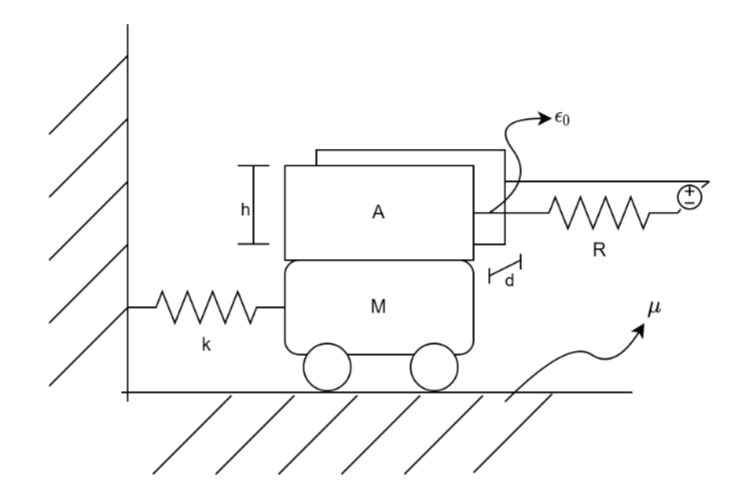
\includegraphics[width=0.6\textwidth]{Auxiliar_6_1}
    \caption{Sistema Electromecánico}
  \end{figure}

  Se tiene un sistema electromecánico que simula el comportamiento de un variador de frecuencia utilizado típicamente en radios de automóviles. En esta ocasión, se le pide simular que el condensador no logra sintonizar la radio de manera constante, sino que oscila respecto al valor nominal de frecuencia para el cual está sintonizado. Su tarea es encontrar la relación que gobierna el voltaje de salida en el condensador que finalmente representa la señal recibida.
%----------------------------
\begin{solution}

\subsection*{Resolución 3.1}

El sistema electromecánico presentado simula el comportamiento de un variador de frecuencia, como los utilizados en radios de automóviles. En este caso, se requiere modelar la situación en la que el condensador no logra sintonizar la radio de manera constante, sino que oscila alrededor del valor nominal de frecuencia para el cual está ajustado. El objetivo es encontrar la relación que gobierna el voltaje de salida en el condensador, el cual representa la señal recibida.

Para abordar este problema, es necesario obtener las ecuaciones de estado que describen el sistema. Utilizaremos el formalismo lagrangiano para la parte mecánica y las leyes de circuitos para la parte eléctrica.
\begin{equation}
\mathcal{L} = T - U = \frac{1}{2}m\dot{x}^2 - \left( \frac{1}{2}C(x)V^2 + \frac{1}{2}k x^2 \right)
\end{equation}
donde $T$ es la energía cinética y $U$ la energía potencial (incluyendo la energía almacenada en el condensador y el resorte). Luego, la capacitancia variable se expresa como
\begin{equation}
C(x) = \frac{\varepsilon_0 (A - |x| h)}{d}
\end{equation}
donde $A$ es el área, $h$ una constante geométrica y $d$ la distancia entre placas.

	extbf{3. Ecuación de Lagrange:}
\begin{equation}
\frac{d}{dt}\left( \frac{\partial \mathcal{L}}{\partial \dot{x}} \right) - \frac{\partial \mathcal{L}}{\partial x} = F_{\text{ext}}
\end{equation}
Calculando las derivadas:
\begin{align}
\frac{\partial \mathcal{L}}{\partial \dot{x}} &= m\dot{x} \\
\frac{d}{dt}\left( \frac{\partial \mathcal{L}}{\partial \dot{x}} \right) &= m\ddot{x} \\
\frac{\partial \mathcal{L}}{\partial x} &= -\frac{\varepsilon_0 x h}{2d|x|} - kx
\end{align}
Por lo tanto la ecuación de movimiento queda:
\begin{equation}
m\ddot{x} - \frac{\varepsilon_0 x h}{2d|x|} + kx = -\mu m g
\end{equation}
donde $-\mu m g$ representa la fuerza de fricción. Luego para el modelo Electrico tenemos:
\begin{figure}[H]
    \centering
    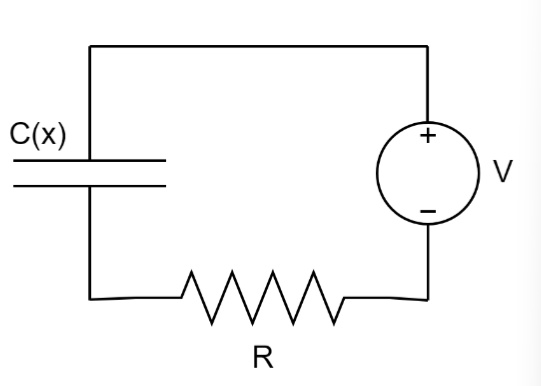
\includegraphics[width=0.4\textwidth]{Auxiliar_6_3}
    \caption{Modelo Electrico}
\end{figure}
Aplicando la Ley de Voltajes de Kirchhoff (LVK) y la relación constitutiva del condensador:
\begin{align}
v_R(t) &= R\,i(t) \\
i(t) &= C(x)\,\frac{dv_C(t)}{dt} \\
V &= v_R(t) + v_C(t)
\end{align}
Sustituyendo $i(t)$ y $C(x)$:
\begin{equation}
V = R\,C(x)\,\frac{dv_C(t)}{dt} + v_C(t) = R\,\frac{\varepsilon_0}{d}(A - |x| h)\,\frac{dv_C(t)}{dt} + v_C(t)
\end{equation}
Finalmente, el sistema completo queda descrito por:
\begin{align}
m\ddot{x} - \frac{\varepsilon_0 x h}{2d|x|} + kx &= -\mu m g \\
V &= R\,\frac{\varepsilon_0}{d}(A - |x| h)\,\frac{dv_C(t)}{dt} + v_C(t)
\end{align}

Estas ecuaciones constituyen el modelo no lineal acoplado del sistema electromecánico, donde la dinámica mecánica y eléctrica están relacionadas a través de la posición $x$ y el voltaje en el condensador $v_C(t)$. La ecuación de movimiento (parte mecánica).
\begin{equation}
m\ddot{x}-\frac{\varepsilon_{0}\,x\,h}{2d|x|}+k x=-\mu m g.
\end{equation}

\textbf{Modelo eléctrico y LVK.} Para relacionar el estado $x$ con el voltaje de salida en el condensador, usamos las leyes constitutivas y la LVK:
\begin{align}
v_{R}(t)&=R\,i(t),
&\qquad
i(t)&=C(x)\,\frac{dv_{C}(t)}{dt},
\\
V&=v_{R}(t)+v_{C}(t).
\end{align}
Sustituyendo $i(t)$ y $C(x)$:
\begin{align}
V&=R\,C(x)\,\frac{dv_{C}(t)}{dt}+v_{C}(t),
\\
V&=R\,\frac{\varepsilon_{0}}{d}\,\big(A-|x|\,h\big)\,\frac{dv_{C}(t)}{dt}+v_{C}(t).
\end{align}

\textbf{Modelo no lineal acoplado del sistema.} Reuniendo ambas partes, el sistema queda:
\begin{align}
m\ddot{x}-\frac{\varepsilon_{0}\,x\,h}{2d|x|}+k x&=-\mu m g, \\[4pt]
V&=\dot{v}_{C}(t)\,R\,\frac{\varepsilon_{0}}{d}\big(A-|x|\,h\big)+v_{C}(t).
\end{align}

\end{solution}

%----------------------------
  \question Considere el circuito de la siguiente figura
  \begin{figure}[H]
    \centering
    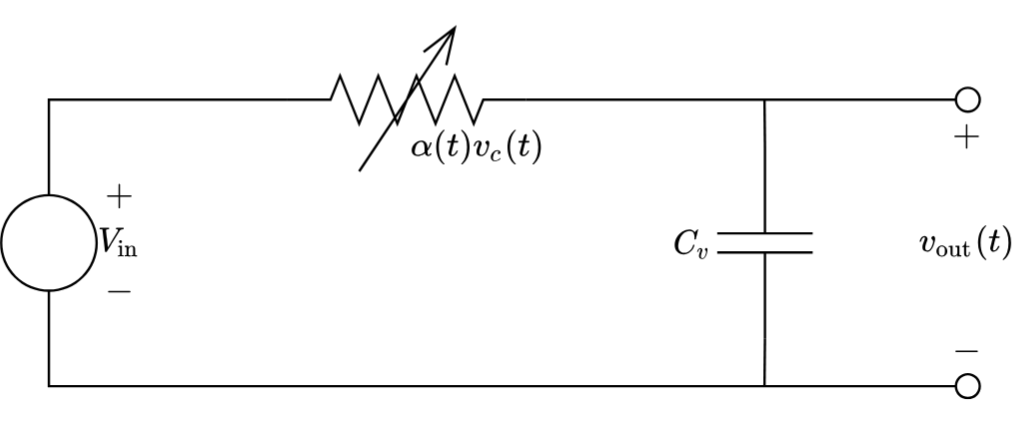
\includegraphics[width=0.6\textwidth]{Auxiliar_6_2}
  \end{figure}

  donde $V_{in} = 10\,$V y $C_v = 1\,$mF.

  \begin{enumerate}
    \item Encuentre las ecuaciones de estado que modelan al sistema.
    \item Determine estado, entrada y salida.
    \item Encuentre estados cero, equilibrio y tierra (en caso de existir).
    \item Linealice el sistema en torno al punto de equilibrio, y formule en variables de estado.
    \item Calcule la MTE y funciones base.
    \item Determine estabilidad Lyapunov, BIBS y BIBO.
    \item Determine la constante de tiempo dominante de la RENC.
    \item Determine controlabilidad y observabilidad.
    \item Diseñe un observador que le permita estimar el estado a partir de la salida.
  \end{enumerate}
%----------------------------
\begin{solution}

\subsection*{Resolución 4.1}

Para modelar el sistema, partimos de la aplicación de la Ley de Voltajes de Kirchhoff (LVK) al lazo del circuito. Al recorrer el lazo, se obtiene:
\begin{equation}
V_{in} = \alpha(t)\,v_c(t)\,i(t) + v_c(t),
\end{equation}
donde $i(t)$ es la corriente en el lazo y el término $\alpha(t)v_c(t)$ representa la resistencia variable del potenciómetro. Por la ley constitutiva del condensador:
\begin{equation}
i(t) = C_v\,\frac{dv_c}{dt},
\end{equation}
donde $C_v$ es la capacitancia y $v_c(t)$ el voltaje en el condensador. Sustituyendo $i(t)$ en la ecuación de LVK, se obtiene:
\begin{align}
V_{in} &= \alpha(t)\,v_c(t)\,C_v\,\frac{dv_c}{dt} + v_c(t) \\
&\implies \alpha(t)\,v_c(t)\,C_v\,\frac{dv_c}{dt} = V_{in} - v_c(t) \\
&\implies \frac{dv_c}{dt} = \frac{V_{in} - v_c(t)}{\alpha(t)\,v_c(t)\,C_v}
\end{align}

Esta es la ecuación diferencial que modela la dinámica del voltaje en el condensador, y constituye la ecuación de estado del sistema.

\subsection*{Resolución 4.2}

Podemos determinar que el estado corresponde a $v_c(t)$, lo cual se justifica porque es la variable que se está derivando. Además, podemos determinar que la \emph{entrada} al sistema es $\alpha(t)$, ya que es el único término que se puede manipular de manera exógena y, considerando que $v_{out}(t)=v_c(t)$, la \emph{salida} corresponde a $v_c(t)$.

Por lo tanto,
\begin{equation}
\boxed{\,x(t)=v_c(t), \qquad u(t)=\alpha(t), \qquad y(t)=v_c(t)=x(t).\,}
\end{equation}

\subsection*{Resolución 4.3}

Para encontrar todos estos estados, consideraremos que $u(t)=0$ (es decir, el análisis se realiza a entrada cero).
\begin{itemize}
  \item  \textbf{Estado cero.} Dado que para este sistema se cumple $y(t)=x(t)$, podemos ver que el estado cero corresponde a $\boxed{x_{\theta}=0}$.

\item \textbf{Estado de equilibrio.} Buscamos $x_e$ tal que $\dot{x}(t)=0$. Evaluando esta condición en la ecuación (3), tenemos
\begin{equation}
V_{in}-v_c(t)\;\Rightarrow\; \boxed{x_e=V_{in}}.
\end{equation}

\item \textbf{Estado tierra.} Del conocimiento previo sobre condensadores, sabemos que en tiempo infinito el condensador se carga y no deja pasar corriente. Teniendo esto en consideración, se cumpliría
\end{itemize}
\begin{equation}
\boxed{x_t=V_{in}}.
\end{equation}

\subsection*{Resolución 4.4}

Para linealizar, consideremos el punto de operación $\bar{x}=V_{in}$ y, para la entrada, $\bar{u}=1$ (ya que $u=0$ haría que hubiera una división por cero).

Si consideramos $F\,(v_c,\alpha)$ como
\begin{equation}
\dot{v}_c(t)=F(v_c,\alpha)=\frac{V_{in}}{\alpha v_c C_v}-\frac{1}{\alpha C_v},
\end{equation}
entonces, para linealizar derivamos respecto a cada término y evaluamos en el punto de operación:
\begin{align}
A
=\left.\frac{\partial F}{\partial v_c}\right|_{V_{in},1}
&=-\left.\frac{V_{in}}{\alpha v_c^{2} C_v}\right|_{V_{in},1}
=-\frac{1}{V_{in} C_v},\\[4pt]
B
=\left.\frac{\partial F}{\partial \alpha}\right|_{V_{in},1}
&=-\left.\frac{V_{in}}{\alpha^{2} v_c C_v}\right|_{V_{in},1}
+\left.\frac{1}{\alpha^{2} C_v}\right|_{V_{in},1}
=-\frac{1}{C_v}+\frac{1}{C_v}=0.
\end{align}

Definiendo $\tilde{x}:=x-\bar{x}$ y $\tilde{u}:=u-\bar{u}$, la ecuación de estado linealizada queda
\begin{align}
\dot{\tilde{x}}&=A\,\tilde{x}+B\,\tilde{u}=-\frac{1}{V_{in}C_v}\,\tilde{x},\\
y&=\tilde{x},
\end{align}
donde $u$ no incide sobre este estado linealizado ($B=0$). Como la salida ya es una ecuación lineal, podemos plantear $y=\tilde{x}$.

Para simplificar notación, reemplazamos $x$ por $\tilde{x}$ (y $y$ por $\tilde{x}$). El sistema linealizado queda
\begin{align}
\dot{x}&=-\frac{1}{V_{in}C_v}\,x,\\
y&=x.
\end{align}

\subsection*{Resolución 4.5}

En general, la matriz de transición de estados es
\begin{equation}
\Phi(t)=e^{At}.
\end{equation}
Dado que en este caso $A$ es un escalar, se obtiene directamente
\begin{equation}
\boxed{\,\Phi(t)=e^{-\frac{t}{V_{in}C_v}}.}
\end{equation}

Para las \emph{funciones base}, notemos que la RENC está dada por
\begin{equation}
y_{0}(t)=C\,\Phi(t)\,x(0).
\end{equation}
Como $C=1$, resulta
\begin{equation}
y_{0}(t)=x(0)\,e^{-\frac{t}{V_{in}C_v}}.
\end{equation}
La única componente linealmente independiente existente es $e^{-\frac{t}{V_{in}C_v}}$, por lo que
\begin{equation}
\boxed{\,\phi=\left\{e^{-\frac{t}{V_{in}C_v}}\right\}.}
\end{equation}

\subsection*{Resolución 4.6}

Para confirmar estabilidad BIBS, basta verificar que los valores propios del sistema tengan parte real negativa. Aquí $A=-\frac{1}{V_{in}C_v}$; considerando que $V_{in}$ y $C_v$ son constantes positivas, el valor propio es $\lambda=-\frac{1}{V_{in}C_v}<0$. Por lo tanto, el sistema es BIBS estable. Al ser BIBS estable (y el sistema lineal e invariante), también es Lyapunov estable y BIBO estable.

\subsection*{Resolución 4.7}

Para una función exponencial $f(t)=e^{-t/\tau}$, la constante de tiempo es $\tau$. Dado que la RENC es
\begin{equation}
y_{0}(t)=x(0)\,e^{-\frac{t}{V_{in}C_v}},
\end{equation}
la constante de tiempo dominante es
\begin{equation}
\boxed{\,\tau=V_{in}C_v.}
\end{equation}

\subsection*{Resolución 4.8}

La matriz de controlabilidad para un sistema SISO de orden $n$ es
\begin{equation}
\zeta=\big[B\;\; AB\;\; A^{2}B\;\; \cdots\;\; A^{n-1}B\big].
\end{equation}
En nuestro caso $n=1$ y $B=0$, por lo que $\zeta=0$ y $\mathrm{rank}(\zeta)=0\neq n$. Concluimos que el sistema \textbf{no es controlable}.

La matriz de observabilidad es
\begin{equation}
\vartheta=
\begin{bmatrix}
C\\
CA\\
CA^{2}\\
\vdots\\
CA^{n-1}
\end{bmatrix}.
\end{equation}
Con $n=1$ se reduce a $\vartheta=C=1$, por lo que $\mathrm{rank}(\vartheta)=1=n$. Concluimos que el sistema \textbf{es observable}.

\subsection*{Resolución 4.9}

De cursos anteriores, la evolución del error en el estimador está dada por
\begin{equation}
\dot{e}=(A-FC)\,e,
\end{equation}
donde $F$ es la ganancia del observador. En general se ubican los polos del error (valores propios de $A-FC$) $\approx$ tres veces más negativos que los del sistema. Aquí el polo del sistema es $-\frac{1}{V_{in}C_v}$; por lo tanto, deseamos
\begin{equation}
A-FC=-\frac{3}{V_{in}C_v}.
\end{equation}
Como $A=-\frac{1}{V_{in}C_v}$ y $C=1$, resulta
\begin{align}
-\frac{1}{V_{in}C_v}-F
&=-\frac{3}{V_{in}C_v}
\quad\Rightarrow\quad
\boxed{\,F=\frac{2}{V_{in}C_v}.}
\end{align}

\end{solution}

\end{questions}
\end{document}